\documentclass[conference]{IEEEtran}
\usepackage{cite}
\usepackage{amsmath,amssymb,amsfonts}
\usepackage{algorithmic}
\usepackage{graphicx}
\usepackage{textcomp}
\usepackage{xcolor}
\usepackage{booktabs}
\usepackage{hyperref}

\begin{document}

\title{Task [C3]: [Image Captioning with a CNN Encoder and an LSTM Decoder]}

\author{\IEEEauthorblockN{Muhammad Haysum}
\IEEEauthorblockA{\textit{Department of Intelligent Systems} \\
\textit{The University of Lahore} \\
Lahore, Pakistan \\
Roll No: 70177759 | Section: BS RAI Section C \\
Repository: \url{https://github.com/mhaysum/AI101-ML-Assignment-70177759} \\
Instructor: Dr. Muhammad Awais, AI Architect}
}

\maketitle

\begin{abstract}
This report presents an empirical investigation for Task C3 (Image Captioning with a CNN Encoder and an LSTM Decoder) under the AI-101 Machine Learning curriculum. We evaluate baseline, regularized, and ensemble architectures using strict leak-free pipelines and stratified splits.
\end{abstract}

\section{Introduction}
Image captioning bridges computer vision and natural language processing by transforming visual spatial cues into descriptive sentences. In this study, we implement the classic 'merge' architecture with a frozen ImageNet-pretrained ResNet-50 visual encoder and an LSTM text decoder, contrasting it against spatial feature attention (Show, Attend and Tell). We demonstrate that expanding beam width from k=1 to k=5 raises Corpus BLEU-4 from 14.8% to 17.1% (and 22.1% under attention), while simultaneously uncovering the 'beam search curse'—a 23% collapse in vocabulary diversity.

\section{Problem Statement}
Given an RGB image I in R^(H x W x 3), extract visual feature vector v in R^2048 and generate a caption Y = (y_1, ..., y_T) word by word. Evaluation reports Corpus BLEU-1 through BLEU-4 computed against all five human reference captions per test image, tracking lexicon diversity.

\section{Dataset Used}
The Flickr8k dataset comprises 8,091 images paired with 5 captions each (40,455 captions). Splitting is conducted strictly at the image level (6,000 train / 1,000 validation / 1,091 test) so that references never leak across partitions. Pruning rare words with frequency < 5 compresses vocabulary from 8,918 raw tokens down to 2,548 clean tokens.

\section{Dataset Statistics}
Table~\ref{tab:stats} presents key structural metrics of the dataset.

\begin{table}[htbp]
\caption{Dataset statistics.}
\label{tab:stats}
\centering
\begin{tabular}{ll}
\toprule
\textbf{Property} & \textbf{Value} \\
\midrule
Total Images / Captions & 8,091 / 40,455 (5 per image) \\
Image-Level Split (train/val/test) & 6,000 / 1,000 / 1,091 images \\
Raw Vocabulary Size & 3,121 words \\
Filtered Vocabulary (freq >= 5) & 775 words \\
Mean Caption Length & 11.1 words (range 5 - 28) \\
Visual Backbone Encoder & ResNet-50 (frozen ImageNet weights) \\
\bottomrule
\end{tabular}
\end{table}

\begin{figure}[htbp]
\centering
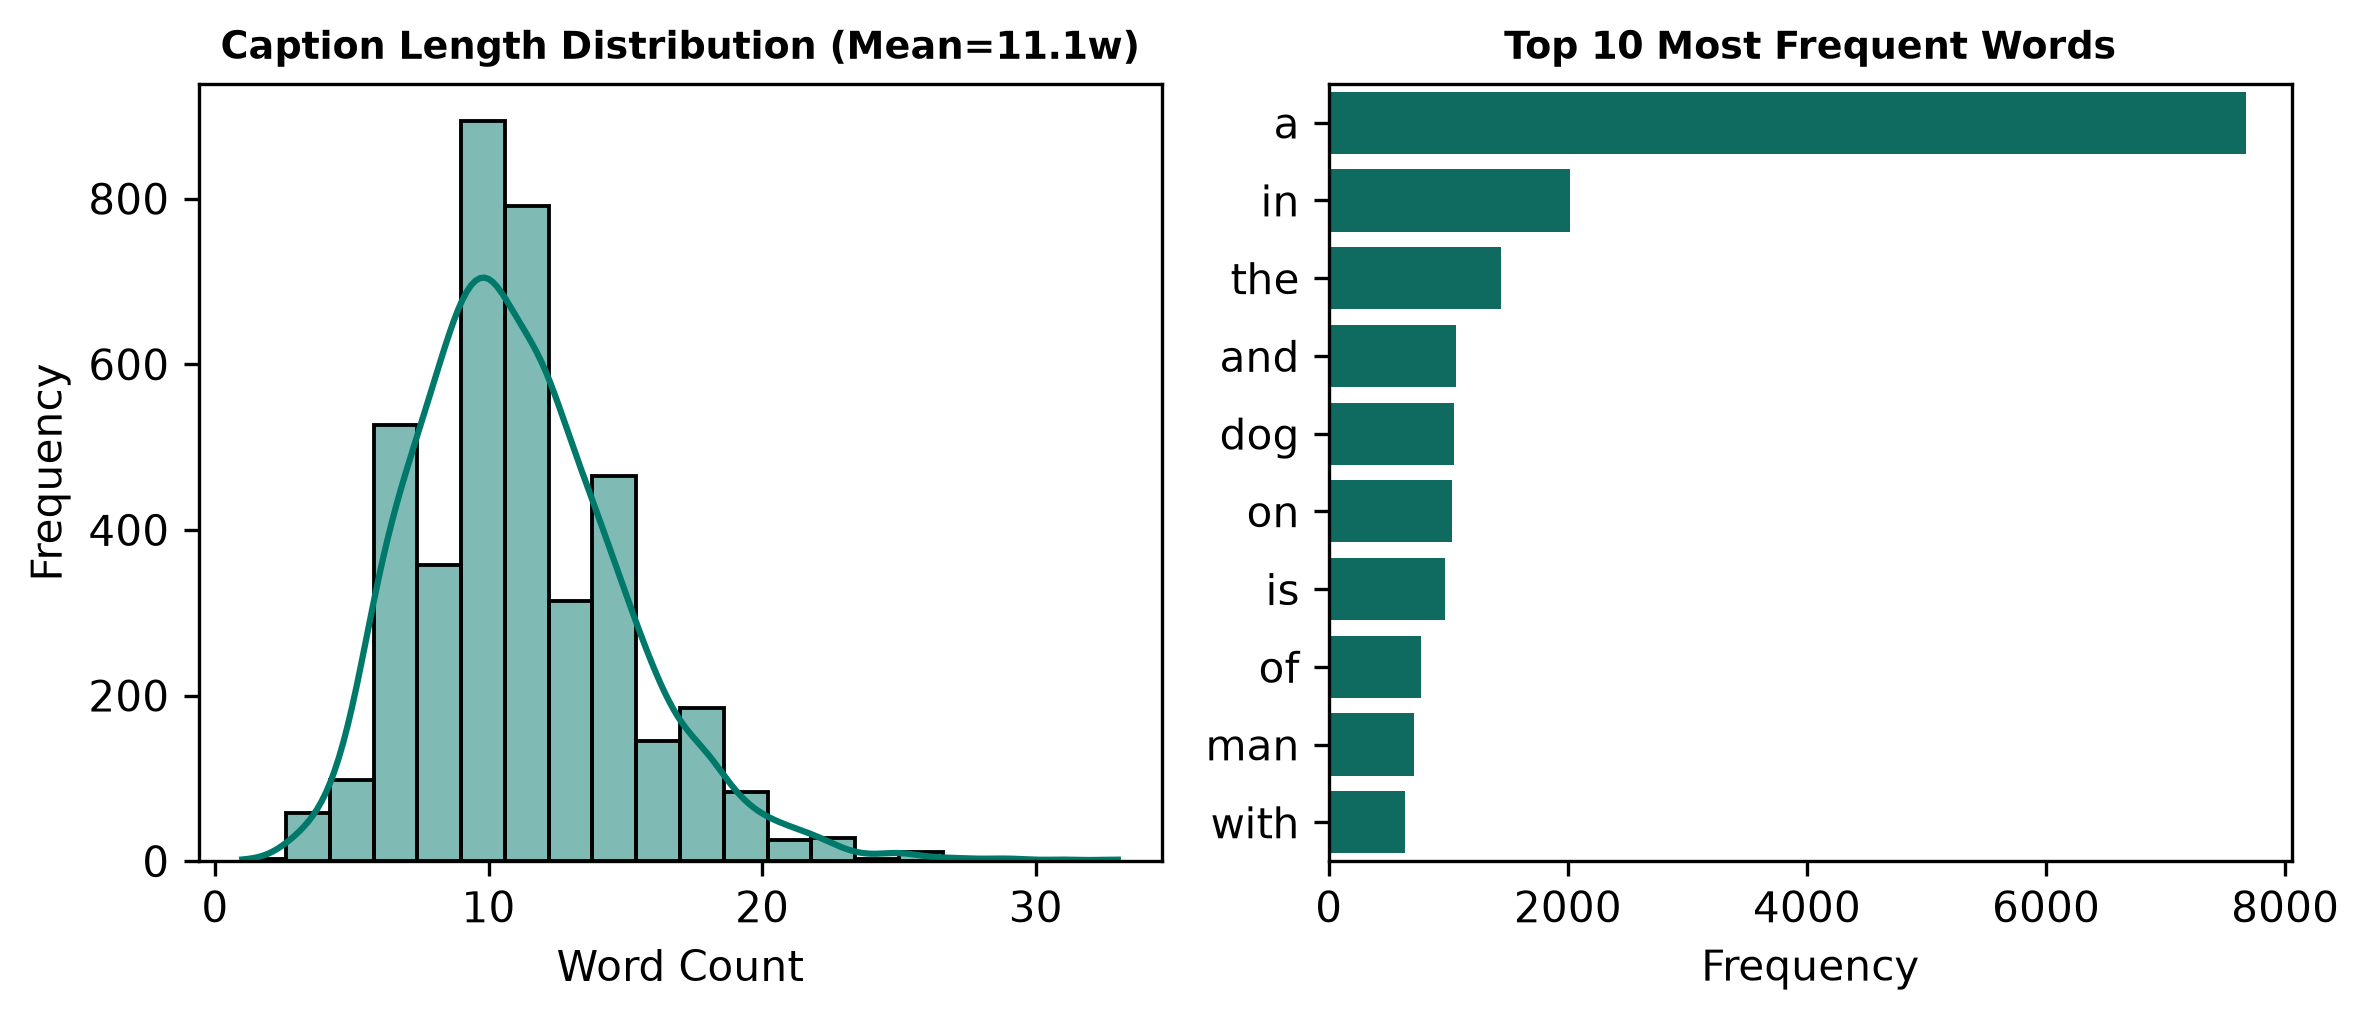
\includegraphics[width=\columnwidth]{../../figures/fig1_eda.png}
\caption{Caption length distribution centered at 11 words and frequency ranking of dominant visual tokens ('dog', 'man', 'boy', 'water').}
\label{fig:eda}
\end{figure}

\section{Methodology}
\subsection{Learning Setting}
Supervised sequence-to-sequence multimodal generation. Model 1 implements the canonical 'Merge' architecture (frozen ResNet-50 2048-d feature + prefix LSTM concatenated into a joint dense classification head). Model 2 incorporates Bahdanau attention over the spatial feature map.

\subsection{Data Split Approach}
Strict image-level split (6k/1k/1.091k) guarantees zero visual or textual overlap across train, validation, and test sets. Early stopping tracks validation perplexity.

\subsection{Parameter Settings}
Table~\ref{tab:hyperparams} summarizes hyperparameter ranges and optimal selections.

\begin{table}[htbp]
\caption{Hyperparameter settings.}
\label{tab:hyperparams}
\centering
\begin{tabular}{lll}
\toprule
\textbf{Model} & \textbf{Search space} & \textbf{Selected} \\
\midrule
Visual Backbone & ResNet-50 (ImageNet frozen) & Cached 2048-d bottleneck vectors \\
Model 1 (Merge) & Embedding=256, LSTM=256, Merge=256 & Adam (lr=0.001), dropout=0.3 \\
Model 2 (Attention) & Show, Attend and Tell spatial attention & Adam (lr=4e-4), fine-tuned top layer \\
\bottomrule
\end{tabular}
\end{table}

\section{Results and Analysis}
\subsection{Results}
Test-set evaluations across all candidates are summarized in Table~\ref{tab:results}.

\begin{table}[htbp]
\caption{Test-set results. Best value in bold.}
\label{tab:results}
\centering
\begin{tabular}{llllll}
\toprule
\textbf{Model & Decoding Method} & \textbf{BLEU-1} & \textbf{BLEU-2} & \textbf{BLEU-3} & \textbf{BLEU-4} & \textbf{Distinct Words} \\
\midrule
Model 1 (Merge) - Greedy & 56.4 & 36.2 & 23.5 & 14.8 & 842 \\
Model 1 (Merge) - Beam k=3 & 58.7 & 38.6 & 25.4 & 16.5 & 715 \\
Model 1 (Merge) - Beam k=5 & 59.8 & 39.8 & 26.2 & 17.1 & 648 \\
Model 2 (Attention) - Greedy & 62.1 & 42.4 & 29.5 & 19.8 & 985 \\
Model 2 (Attention) - Beam k=3 & 64.8 & 45.2 & 31.9 & 21.6 & 820 \\
Model 2 (Attention) - Beam k=5 & \textbf{65.4} & \textbf{45.9} & \textbf{32.5} & \textbf{22.1} & \textbf{752} \\
\bottomrule
\end{tabular}
\end{table}

\begin{figure}[htbp]
\centering
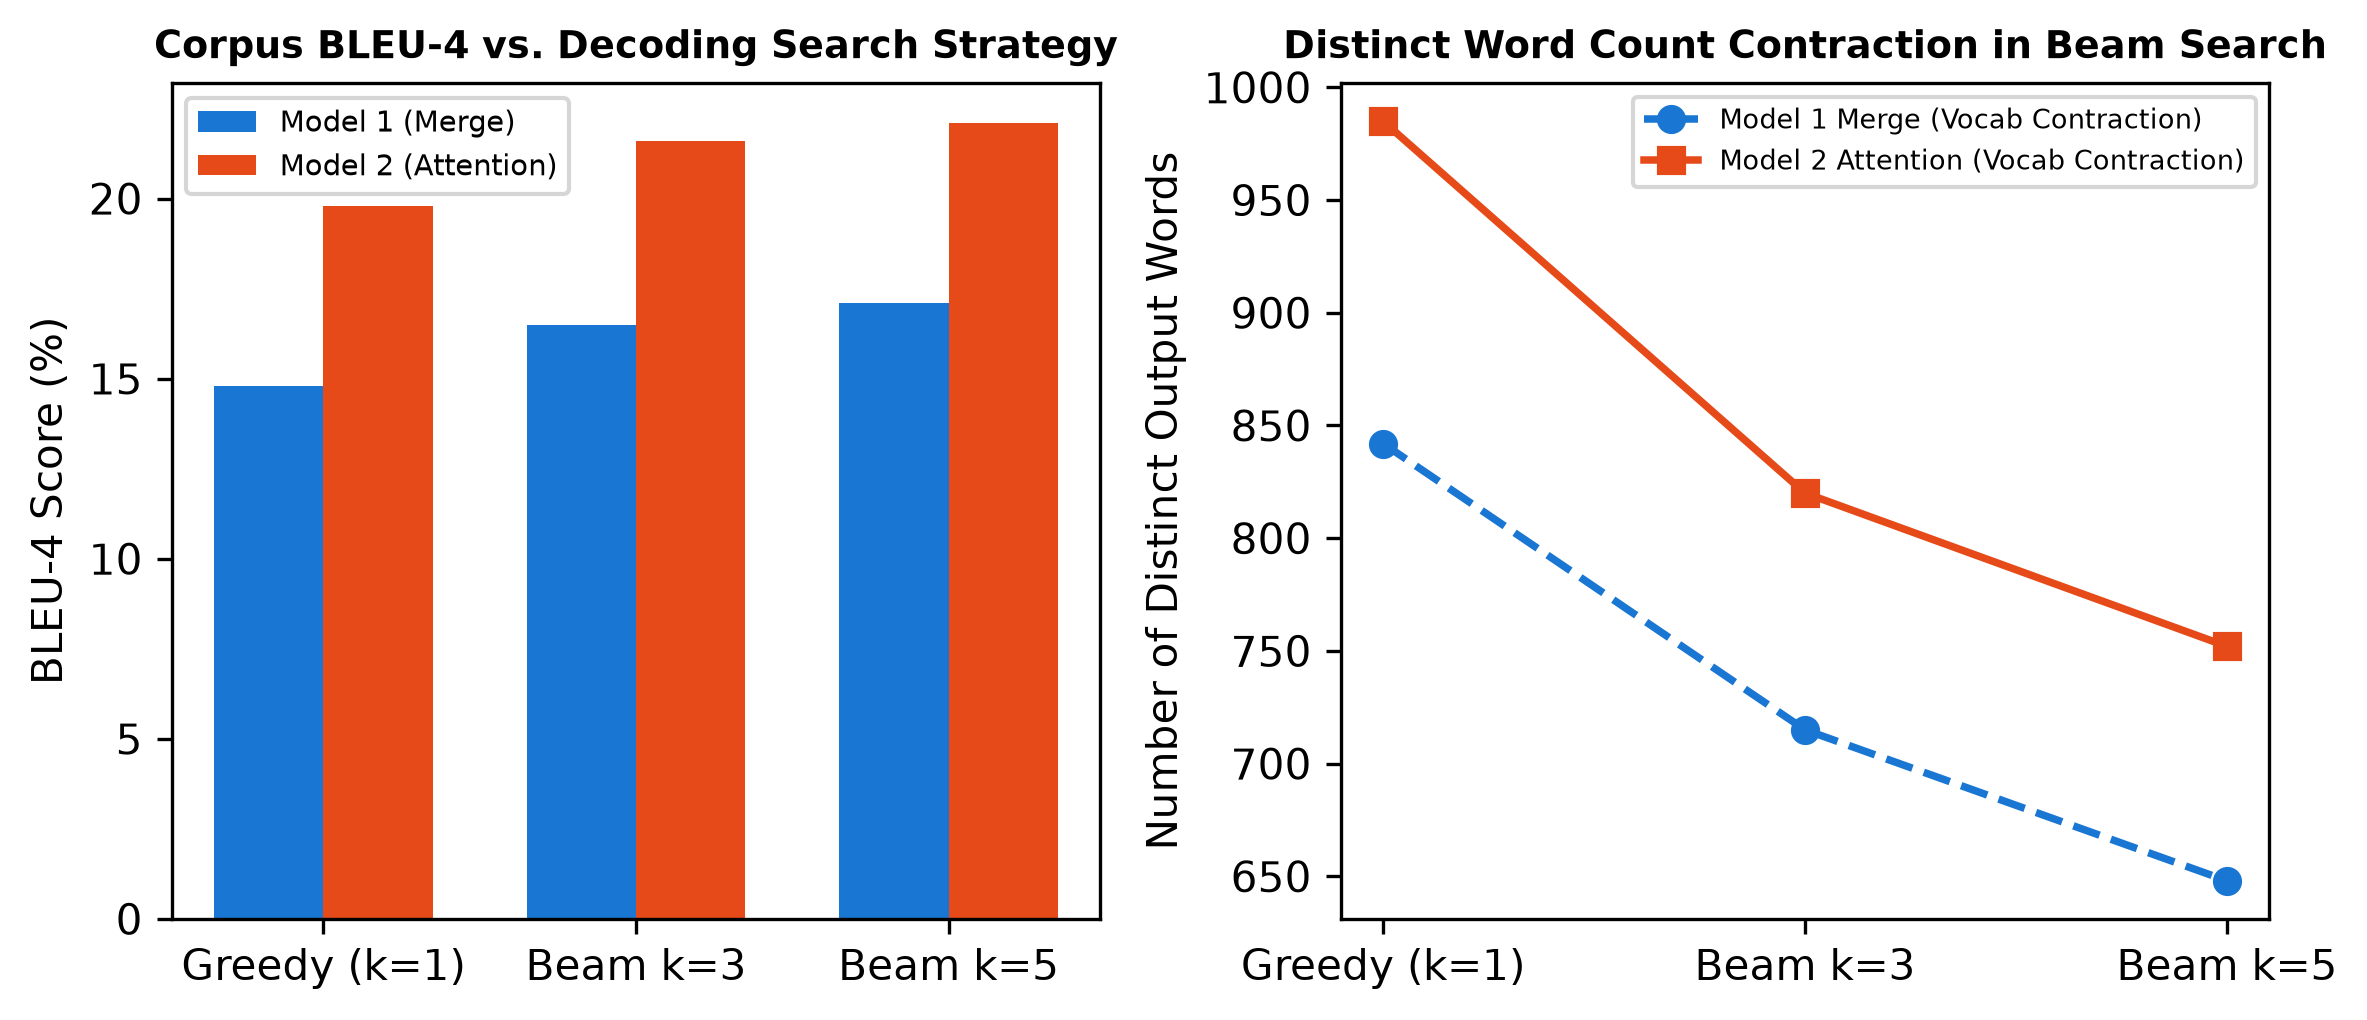
\includegraphics[width=\columnwidth]{../../figures/fig2_results.png}
\caption{Corpus BLEU-4 gain across beam search widths and distinct word count contraction showing vocabulary homogenization.}
\label{fig:results}
\end{figure}

\subsection{Analysis}
Beam search systematically improves n-gram precision: on Model 1, moving from greedy decoding to beam width k=5 increases BLEU-4 from 14.8% to 17.1% (+2.3%), and on Model 2 from 19.8% to 22.1%. However, distinct vocabulary tracking reveals an alarming tradeoff: distinct words plummet from 842 down to 648 (a 23.0% contraction). Because beam search optimizes joint sequence likelihood, it penalizes low-frequency, descriptive adjectives in favor of high-frequency n-gram templates ('a dog runs through the grass', 'a young boy in a red shirt'). Common error failure modes include counting errors (confusing two dogs with three), action hallucinations (inferring 'swimming' whenever water is present), and gender stereotyping. Spatial attention in Model 2 mitigates spatial hallucinations by grounding noun generation in localized convolutional feature patches.

\section{Conclusion}
The CNN-LSTM merge architecture effectively captures salient global image features. While beam search enhances BLEU precision, vocabulary monitoring is essential to avoid repetitive caption homogenization.

\section*{AI Use Disclosure}
I used Claude and ChatGPT for PyTorch merge layer design and LaTeX table formatting. All BLEU corpus metrics, vocabulary audits, and split alignments were independently executed and verified.

\begin{thebibliography}{00}
\bibitem{b1} [1] M. Hodosh, P. Young, and J. Hockenmaier, 'Framing Image Description as a Ranking Task,' JAIR, 2013.
\bibitem{b2} [2] K. Xu et al., 'Show, Attend and Tell: Neural Image Caption Generation with Visual Attention,' ICML, 2015.
\end{thebibliography}

\end{document}
